%==============================================================================
\section{Overview}
\label{sec:overview}


This section presents the intuition behind \system's approach to efficiently execute graph
queries. We begin by considering a running example from financial fraud detection.

\noindent\textit{Query.} Detect rapid 3-hop transfers of large amounts, where the money starts or ends in newly opened account and moves across different owners.
\begin{verbatim}
    MATCH (a1:Account)-[t1:TXN]->(a2:Account)
      -[t2:TXN]->(a3:Account)-[t3:TXN]->(a4:Account)
    WHERE t1.amount > 10000
      AND t2.amount > 10000
      AND t3.amount > 10000
      AND t2.ts <= t1.ts + duration({minutes: 10})
      AND t3.ts <= t2.ts + duration({minutes: 10})
      AND ( a1.open_date >= date() - duration({days: 30})
        OR a4.open_date >= date() - duration({days: 30}))
      AND a1.owner_id <> a2.owner_id
      AND a2.owner_id <> a3.owner_id
      AND a3.owner_id <> a4.owner_id
    RETURN a1.acc_id, a2.acc_id, a3.acc_id, a4.acc_id
\end{verbatim}

Modeling the above $k=3$-hop query as a general multi-way join results
in $2k+1 = 7$ relations in the join tree, leading to XX sorts. 
Our goal is to design a specialized \emph{one-hop} operator (i.e., $n_i \rightarrow e
\rightarrow n_j$) that significantly reduces this overhead while revealing only the 
size of the edge list, which is public. In contrast to treating a one-hop pattern as a 
three-way join, our operator requires only a single oblivious sort and can be applied in
parallel across the query, as we show in ~\Cref{fig:intuition}. This enables
a hybrid strategy where we process one-hop patterns ($H1$ and $H2$ in the figure)
using the specialized operator, while retaining the general multi-way join framework for the
remaining structure. For the above example, this strategy transforms a 7-way join into
a 3-way join, which significantly brings the execution time of the query, as we experimentally
show in \cref{sec:evaluation}. Apart from reducing the length, the decomposition approach
enables parallelism and minimizes the amount of sequential processing because \wei cannot process a 
parent node without processing all its children in the bottom-up phase, and vice versa in the 
top-down phase.


\begin{figure}
    \centering
    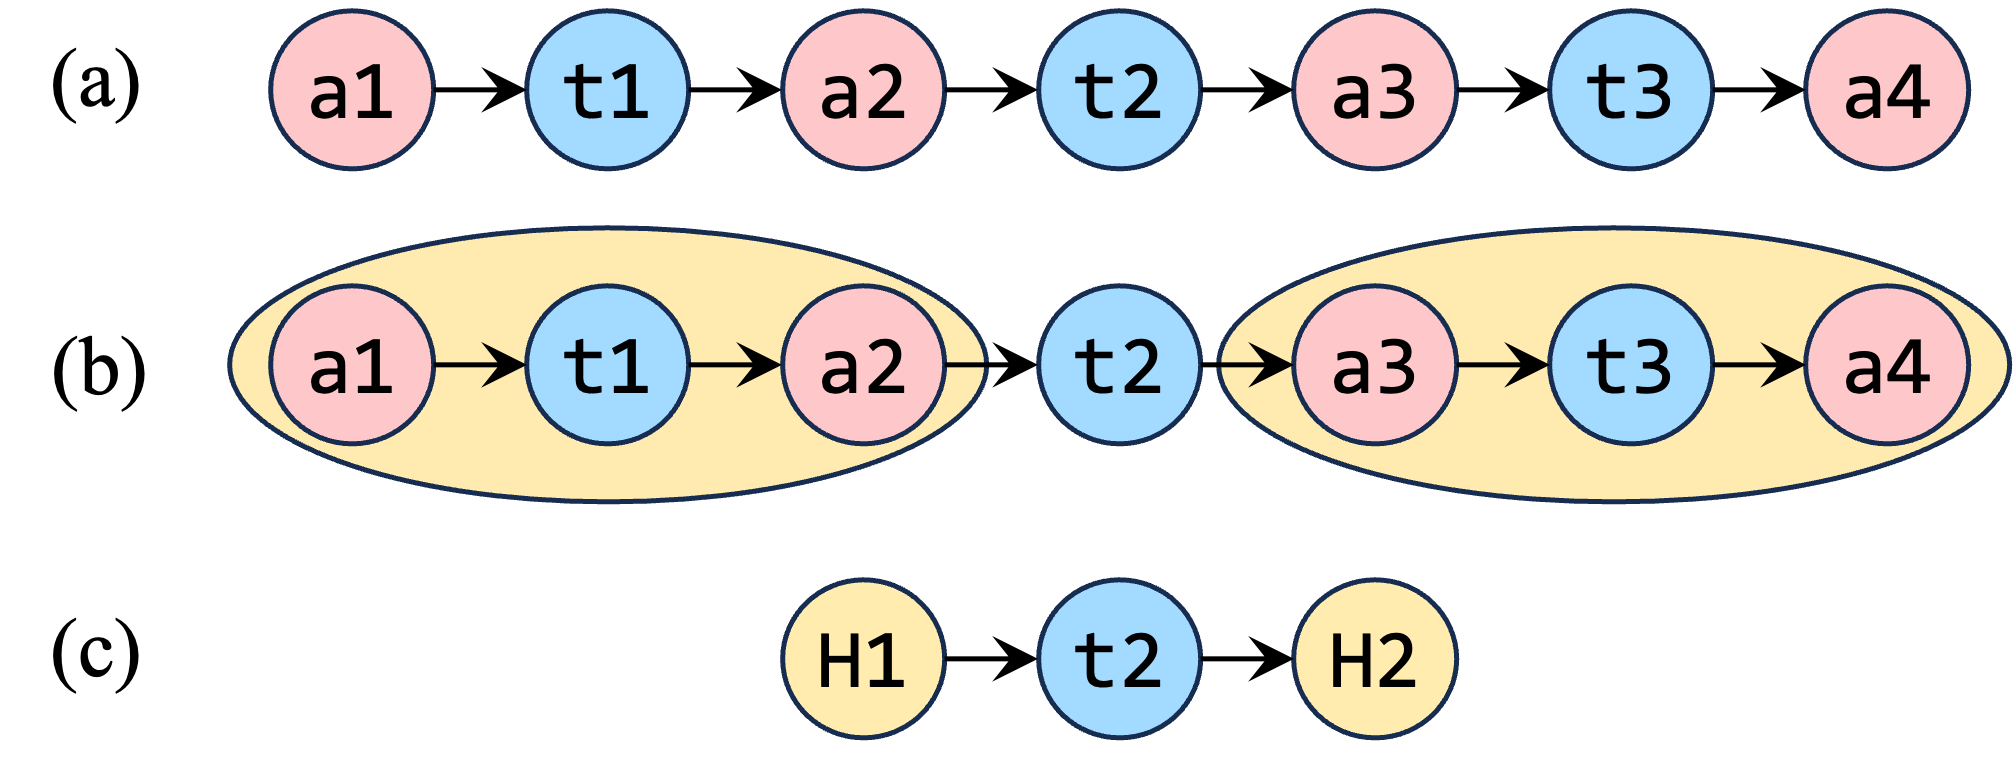
\includegraphics[width=0.7\linewidth]{figures/intuition-example.png}
    \caption{Reducing the length of a graph query}
    \label{fig:intuition}
\end{figure}


Based on the above intuition, \system requires two main components in serving graph queries
apart from integrating \wei: the \onehop operator and a query decomposer, which acts as a
query planner by identifying one-hop patterns and decomposing a long query into parallelizable
components. The next two sections describe the two components in detail.

% \paragraph{Baseline Execution (No Decomposition).}
% Using only the oblivious multi-way join, this query is treated as a three-way join: $\texttt{Account} \bowtie \texttt{Transaction} \bowtie \texttt{Account}$. The algorithm must:
% \begin{enumerate}
%     \item Build a join tree with three nodes
%     \item Execute bottom-up phase: compute multiplicities for all tuples
%     \item Execute top-down phase: replicate and align tuples
%     \item Apply the filter \texttt{a1.balance > 10000} obliviously
% \end{enumerate}
% This requires multiple oblivious sorts over the combined data.

% \paragraph{Optimized Execution (With \system).}
% The query decomposer recognizes this as a single one-hop pattern and routes it entirely to the \onehop operator:
% \begin{enumerate}
%     \item Build oblivious hash map for \texttt{Account} (filtered by balance $> 10000$)
%     \item Sort \texttt{Transaction} by \texttt{src\_id}
%     \item Apply duplicate suppression: mark first occurrence of each \texttt{src\_id}
%     \item Probe hash map for marked entries only
%     \item Forward-fill: propagate results to all transactions with same source
%     \item Repeat for destination side
%     \item Output: 50,000 rows (padded with dummies for non-matches)
% \end{enumerate}

% The key difference: \onehop avoids the full multi-way join machinery by exploiting the graph structure. The output size (50,000 = $|$\texttt{Transaction}$|$) is public, so no information leaks.

% \paragraph{Multi-Hop Example.}
% For longer queries like a 3-hop chain:
% \begin{center}
% \small
% \texttt{(a1:Account)-[t1]$\rightarrow$(a2)-[t2]$\rightarrow$(a3)-[t3]$\rightarrow$(a4:Account)}\\
% \texttt{WHERE a1.balance > 10000 AND a4.balance < 1000}
% \end{center}

% The decomposer identifies two optimizable one-hop patterns (at the endpoints where filters exist) and rewrites the query:
% \begin{enumerate}
%     \item $H_1$ = \onehop(\texttt{a1}, \texttt{t1}, \texttt{a2}) with filter on \texttt{a1}
%     \item $H_2$ = \onehop(\texttt{a3}, \texttt{t3}, \texttt{a4}) with filter on \texttt{a4}
%     \item Reduced query: $H_1 \bowtie \texttt{t2} \bowtie H_2$
% \end{enumerate}

% The reduced query has only 3 tables instead of 7, significantly reducing the work for the oblivious multi-way join.


% %==============================================================================

% This section presents the architecture of \system and illustrates its operation through a running example.

% %------------------------------------------------------------------------------
% \subsection{Architecture}
% \label{sec:overview:arch}
% %------------------------------------------------------------------------------

% We consider a system model where an organization outsources its storage and computational needs to a 
% cloud. The organization uploads encrypted graph data to the cloud and issues queries to \system hosted
% within a secure enclave in the cloud. Figure~\ref{fig:architecture} shows the architecture of \system's
% query processing engine. Given a multi-hop graph query, the system processes it through three main components:

% \begin{enumerate}[leftmargin=*]
%     \item \textbf{Query Decomposer} (Section~\ref{sec:decomposition}): Analyzes the graph query to identify one-hop patterns and rewrite the original query into a combination of one-hop operators wherever possible.

%     \item \textbf{\Onehop Operator} (Section~\ref{sec:onehop}): Executes our novel
%     oblivious one-hop processing algorithm. Each one-hop operation produces output with size equal to 
%     the edge table, which is a publicly known quantity.

%     \item \textbf{Oblivious Multi-Way Join Operator}~\cite{ruidi2025oblivious}: Handles the reduced query after one-hop operations complete. This component uses existing oblivious join algorithms to process the remaining joins while hiding intermediate result sizes.
% \end{enumerate}

% \begin{figure}[t]
% \centering
% \small
% \includesvg[width=0.6\columnwidth]{figures/system-architecture}
% % 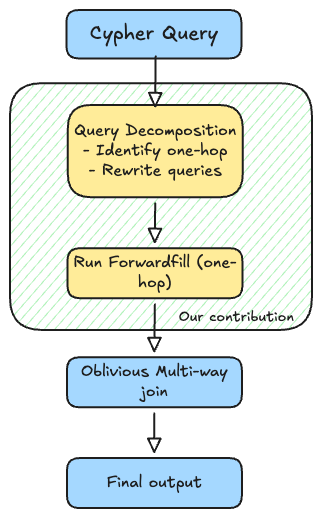
\includegraphics[width=0.85\columnwidth]{figures/system-architecture.png}
% \caption{Architecture of \system. Query decomposition identifies one-hop patterns for optimization. The \onehop operator processes these patterns efficiently, while the oblivious multi-way join handles remaining complexity.}
% \label{fig:architecture}
% \end{figure}

% %------------------------------------------------------------------------------
% \subsection{Key Design Decisions}
% \label{sec:overview:design}
% %------------------------------------------------------------------------------

% Three key design decisions underpin our approach:

% \paragraph{Public-Sized Outputs from One-Hop.}
% The \onehop operator always produces output of size $|E|$, where $E$ is the edge table. Since edge table sizes are public information in our threat model (Section~\ref{sec:background:threat}), this output size reveals nothing new to the adversary. Non-matching tuples are replaced with dummy entries to maintain the fixed size. This property is crucial: it allows us to use faster, graph-native algorithms for one-hop traversals without compromising security.

% \paragraph{Composition with Multi-Way Joins.}
% The outputs of \onehop operations become inputs to the oblivious multi-way join algorithm. Because these outputs have publicly known sizes, the composition remains secure---the multi-way join algorithm's security guarantees hold when all input sizes are public. This modular design allows us to leverage existing, well-analyzed oblivious join algorithms.

% \paragraph{Greedy Decomposition.}
% Our query decomposition uses a greedy strategy to select which one-hop patterns to optimize. While optimal decomposition is NP-hard in general, greedy selection works well for common query patterns (chains, stars, trees) and provides consistent speedups in practice.

% %------------------------------------------------------------------------------
% \subsection{Running Example}
% \label{sec:overview:example}
% %------------------------------------------------------------------------------

